\chapter{Android Usability Study}
\section{Einleitung}
Bei dem Projekt BestShift hat die Android Applikation eine hohe Priorität, weil diese die Daten sammelt, dem Nutzer möglichst in Echtzeit darstellt und sie außerdem auf den Server lädt um Sie dem Nutzer für eine weitere Analyse verfügbar zu machen. 
Daher ist die Android App, neben dem Car-PC, die zentrale Schnittstelle für die Daten die gesammelt werden. 

\section{Design-Überblick}
Das Design ist als Tab-Implementierung umgesetzt worden, was den Fahrer bei der Fahrt möglichst wenig ablenken wird, weil er um zu den unterschiedlichen Funktionen zu gelangen keinen kleinen Knopf erwischen muss, sondern den kompletten Bildschirm seines Smartphones verwenden kann. Innerhalb der einzelnen Views und Activities setzt dann jeder der App-Beteiligten seine eigenen Designs um. 

Diese Umsetzung mittels der Tab-Implementierung sieht bisher so aus.
\newpage
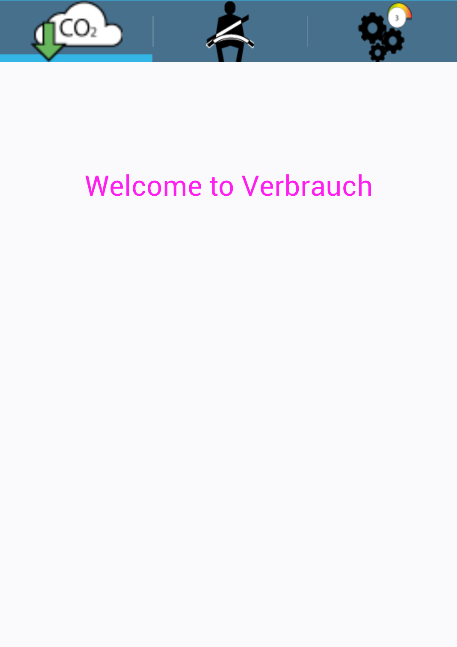
\includegraphics[scale=0.4]{images/Verbrauch.png}
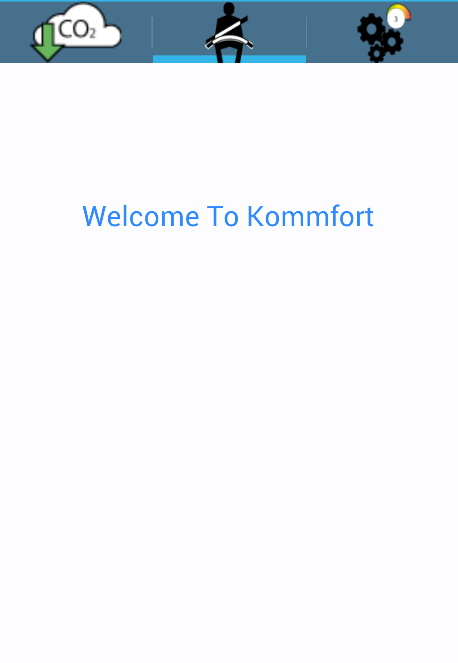
\includegraphics[scale=0.4]{images/Komfort.png}
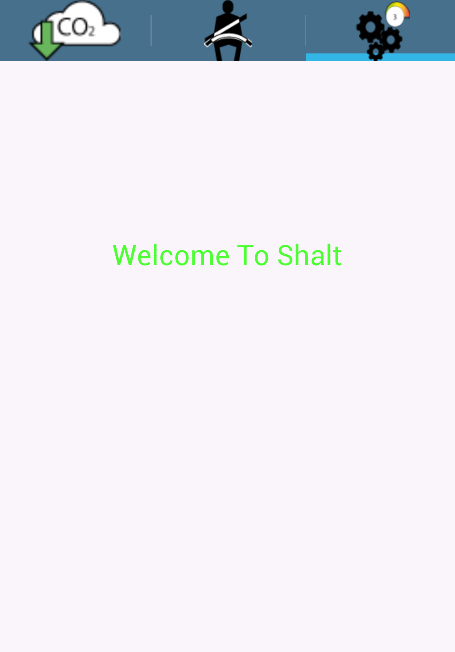
\includegraphics[scale=0.4]{images/Schalt.png}

\newpage
\section{Swipe-Dokumentation}
Wir erstellen erstmal eine MainActivity Klasse in dem wir von FragementActivity erben und von ActionTabListener implementieren um die Methoden onTabReselected, onTabselected und onTabunselected zu überschreiben.  
\newline            
Nachher setzen wir die View der Klasse auf main mit:
\begin{lstlisting}
	setContentView(R.layout.main);	
\end{lstlisting}

\newline
Wir erstellen ein Objekt von ActionBar und fügen mehrere Tabs hinzu, außerdem wird das Layout für die Navigation mittels Tabs so realisiert:
\begin{lstlisting}
// setzen der Navigation für die Tabs
actionbar.setNavigationMode(ActionBar.NAVIGATION_MODE_TABS);
\end{lstlisting}

\newline
Folgend werden mehrere Tabs so hinzugefügt:
\begin{lstlisting}
	// Tabs werden hinzugefügt
actionbar.addTab(actionbar.newTab().setTabListener(this).setIcon(R.drawable.verbrauchwolke));
actionbar.addTab(actionbar.newTab().setTabListener(this).setIcon(R.drawable.komfort), true);// Setzen des Tabs auf angeklickt mit True
actionbar.addTab(actionbar.newTab().setTabListener(this).setIcon(R.drawable.schaltvorschlag));
// Weiters werden Icons zu den Tabs hinzugefügt.
\end{lstlisting}

\newline
Folgend wird das Design mittels der main.xml überarbeitet. Es wird ein ViewPager Layout, welches das Swipen erlaubt, implementiert:
\begin{lstlisting}
	<android.support.v4.view.ViewPager> </android.support.v4.view.ViewPager>
\end{lstlisting}
 Wir übergeben dem Layout ebenfalls eine id auf die wir von unserer main Activity zugreifen:
\begin{lstlisting}
	android:id="@+id/pager"
\end{lstlisting} 

\newline
Nun erstellen wir eine Fragementadapter Klasse um die einzelnen Tabs den jeweiligen Klassen zuzuteilen. 
Die Klasse hat einen Konstruktor welcher von der Superklasse FragementManager ein Objekt übergeben bekommt. Weiters hat die Klasse eine getItem Methode mit dem Input eines int Wertes. 
\begin{lstlisting}
	@Override
    public Fragment getItem(int arg0) {
        switch (arg0) {
            case 0:
                return new Verbrauch();
            case 1:
                return new Kommfort();
            case 2:
                return new Shift();
            default:
                break;
        }
            return null;

    }
\end{lstlisting}
Hier wird nur geprüft welcher Tab angeklickt wurde, dem teilt er einer Klasse mit welche eine eigene View hat.
Sie hat noch eine getCount() Methode welches die Anzahl der Tabs zurück gibt in unserem Fall 3.

\newpage
Wir erstellen auf der Main Klasse zwei Objekte:
\begin{lstlisting}
	ViewPager viewpager;
	FragmentPagerAdapter ft;
	
	viewpager =(ViewPager) findViewById(R.id.pager);
	ft = new FragementPageAdapter(getSupportFragmentManager());

	viewpager.setAdapter(ft);
	//Das Machen wir um zwischen den Oberflächen wechseln zu können.
\end{lstlisting}

\subsection{Oberflächen erstellen}
Nun erstellen wir die Klassen und auch die Layouts für unsere drei Oberflächen, das machen wir indem wir zuerst eine solche übersichtliche Ordnerstruktur erstellen:
\newpage
\dirtree{%
.1 /BestShift-App.
.2 AndroidManifest.xml.
.2 Swipe.iml.
.2 ant.properties.
.2 build.xml.
.2 gen.
.3 com.
.4 BestShift.
.5 app.
.6 BuildConfig.java.
.6 Manifest.java.
.6 R.java.
.2 local.properties.
.2 out.
.3 production.
.4 BestShift.
.5 Swipe.apk.
.5 Swipe.unaligned.apk.
.5 com.
.6 BestShift.
.7 app.
.8 BuildConfig.class.
.8 FragementPageAdapter.class.
.8 Komfort.
.9 Komfort.class.
.8 MyActivity\$ 1.class.
.8 MyActivity.class.
.8 R\$ attr.class.
.8 R\$ drawable.class.
.8 R\$ id.class.
.8 R\$ layout.class.
.8 R\$ string.class.
.8 R.class.
.8 Shift.
.9 Shift.class.
.8 Verbrauch.
.9 Verbrauch.class.
.7 Swipe.
.8 R\$ style.class.
.4 Swipe.
.5 Swipe.apk.
.5 Swipe.unaligned.apk.
.5 com.
.6 BestShift.
.7 app.
.8 BuildConfig.class.
.8 FragementPageAdapter.class.
.8 Komfort.
.9 KammscherKreis\$ 1.class.
.9 KammscherKreis.class.
.9 Komfort\$ 1.class.
.9 Komfort.class.
.8 MyActivity\$ 1.class.
.8 MyActivity.class.
.8 R\$ attr.class.
.8 R\$ drawable.class.
.8 R\$ id.class.
.8 R\$ layout.class.
.8 R\$ string.class.
.8 R.class.
.8 Shift.
.9 Shift.class.
.8 Verbrauch.
.9 Verbrauch.class.
.2 proguard-project.txt.
.2 project.properties.
.2 res.
.3 drawable-hdpi.
.4 ic_launcher.png.
.3 drawable-ldpi.
.4 ic_launcher.png.
.4 komfort.png.
.4 schaltvorschlag.png.
.4 verbrauchwolke.png.
.3 drawable-mdpi.
.4 ic_launcher.png
.3 drawable-xhdpi.
.4 ic_launcher.png
.3 layout.
.4 kammscherkreis.xml.
.4 komfort.xml.
.4 main.xml.
.4 schalt.xml.
.4 verbrauch.xml.
.3 values.
.4 strings.xml.
.2 src.
.3 com.
.4 BestShift.
.5 app.
.6 FragementPageAdapter.java.
.6 Komfort.
.7 KammscherKreis.java.
.7 Komfort.java.
.6 MyActivity.java.
.6 Shift.
.7 Shift.java.
.6 Verbrauch.
.7 Verbrauch.java.
}

\newpage
Wir erstellen die Klasse z.B Komfort welches von einem Fragment erbt. Und hier wird das Komfort-Layout übergeben:
\newline
\begin{lstlisting}
	return inflater.inflate(R.layout.kommfort, container, false);
\end{lstlisting}
